\chapter{Statistiques}

La statistique est la technique des mathématiques qui s’occupe de rassembler, d’organiser, d’analyser et d’interpréter des observations numériques, afin d’en tirer des conclusions les plus justes possible.
Cela présuppose que nous adoptions dans notre démarche de recherches des faits une méthode sûre, une appréciation selon un ordre logique.
Pour rassembler des données, nous pouvons procéder à un dénombrement instantané de toute une population (Ex. des recensements fédéraux qui interviennent tous les dix ans) ou alors - et c’est la méthode adoptée par le “marketing” d’entreprise - par des sondages dans une population donnée. Nous n’effectuerons pas nous-mêmes des sondages, car c’est un travail long, fastidieux et coûteux qui dépasserait largement notre temps disponible en mathématiques. Nous allons, dans notre cours, définir les principaux termes employés en statistique, procéder à l’établissement de tableaux statistiques selon différentes méthodes, étudier les éléments caractéristiques mathématiques de ces données.

\section{Vocabulaire}

Un certain nombre de termes nouveaux sont présents dans toute analyse statistique. Il s’agit des termes suivants :

\begin{definition}
\begin{enumerate}
\item La \emph{population}\index{statistiques!population}, dans une étude statistique, désigne les éléments de l’ensemble étudié. Ce ne sont pas forcément des personnes humaines.
\item La population possède un ou plusieurs traits communs présentés ou non par chacun des éléments ou unités statistiques recensés dans un ensemble donné. Ces traits sont appelés des \emph{caractères}\index{statistiques!caractère} et notés $x_i$.
\item L’\emph{effectif}\index{statistiques!effectif} indique le nombre de membres de la population étudiée qui possèdent le caractère étudié. On le note $n$.
\item Lorsque nous ordonnons et classons les éléments de la population en fonction du caractère, nous obtenons une \emph{distribution statistique}\index{statistiques!distribution}.
\item La \emph{fréquence}\index{statistiques!fréquence} est le rapport entre l’effectif correspondant à un caractère observé et l’effectif total. On la note $f_i$.
\item La \emph{moyenne}~\index{statistiques!moyenne} représente la valeur la plus proche de toutes les valeurs de la distribution.
\item La \emph{médiane}~\index{statistiques!médiane} représente la valeur qui coupe en deux parties de tailles égales la distribution.
\item La \emph{variance}~\index{statistiques!variance} représente l'écart de la distribution par rapport à la moyenne. On la note $v$.
\item L'\emph{écart-type}~\index{statistiques!écart type} représente aussi l'écart de la distribution par rapport à la moyenne, mais de manière plus précise. On le note $\sigma$
\item Le \emph{mode}~\index{statistiques!mode} représente le caractère qui est le plus constaté dans la distribution.
\end{enumerate}
\end{definition}

\begin{remarque}
On peut distinguer deux grandes séries de distributions statistiques :
\begin{itemize}
\item \emph{Distribution statistique discrète}\index{statistiques!distribution discrète} : le caractère ne peut prendre que des valeurs numériques isolées. Par exemple un nombre de points à un examen, un nombre de frères et soeurs, etc.
\item \emph{Distribution statique continue}\index{statistiques!distribution continue} : le caractère peut prendre toutes les valeurs dans un intervalle. Par exemple : une taille, un poids, une vitesse, etc. Dans ce cas, on s'intéressera plus au \emph{centre de classe}~\index{statistiques!Centre de classe}, c'est-à-dire au nombre qui coupe l'intervalle en deux parties égales.
\end{itemize}
Il peut cependant arriver qu'on préfère rassembler des distributions discrètes dans des intervalles pour avoir une meilleures lisibilité. Par exemple, si l'on a relevé la vitesse en $km/h$ (distribution discrète car arrondie) d'une centaine de voitures, on peut décider de les trier par intervalle de $5km/h$.
\end{remarque}

\section{Tableau statistique}

Pour nous aider à visualiser la situation et à déterminer certaines valeurs clefs selon la distribution statistique, nous allons former un \emph{tableau statistique} ayant les colonnes suivantes :
\begin{enumerate}[colonne 1 : ]
\item caractère de la distribution. On va généralement ordonner ceux-ci selon un ordre croissant. Si la distribution est discrète. On notera également le centre de classe dans une colonne $1$bis.
\item effectifs. On donnera l'effectif de la distribution lié à chaque caractère, c'est-à-dire combien de fois chaque caractère apparaît dans notre relevé statistique. On donnera également le \emph{total des effectifs} au fond de la colonne.
\item fréquence. Elle représente le pourcentage d'apparition du caractère dans la série. On la calcule ainsi :
$$
f_i = \frac{n_i}{N} = \frac{\mbox{effectifs du caractère}}{\mbox{effectifs totaux}}.
$$
On peut donner sa valeur soit en $\%$ soit en décimal (ex : $20\%$ ou $0.20$). \textcolor{red}{La somme des fréquences doit toujours être de $100\%$ ou de $1$ car il s'agit de l'ensemble de la distribution.}
\item fréquence cumulée (notée $F_i$)~\index{statistiques!Fréquence cumulée}. Elle représente la somme des fréquences des caractères inférieurs ou égaux, c'est-à-dire le pourcentage de la distribution inférieur ou égal au caractère. On la calcule en additionnant les lignes des fréquences de caractère inférieur ou égal. Ex : pour trouver $F_3$ on fait $f_1 + f_2 + f_3$. On peut également gagner du temps en faisant $F_2 + f_3$.
\item fréquence cumulée inverse (notée $F_i'$)~\index{statistiques!Fréquence cumulée inverse}. Elle représente la somme des fréquences des caractères supérieurs ou égaux, c'est-à-dire le pourcentage de la distribution supérieur ou égal au caractère. On la calcule en additionnant les lignes des fréquences de caractère supérieur ou égal. Ex : pour trouver $F_3'$ sur une distribution à $5$ caractères, on fait $f_3 + f_4 + f_5$. On peut également gagner du temps en faisant $F_4' + f_3$. Il est donc plus intéressant de partir du fond du tableau.
\item fréquence pondérée (notée $f_ix_i$)~\index{statistiques!Fréquence pondérée}. Elle ne représente en soi rien, mais la somme de toutes les fréquences pondérées du tableau donne la moyenne de la distribution. On la calcule en multipliant la fréquence par le caractère (ou par le centre de classe dans une distribution discrète). Ex : si $20\%$ de la classe a fait $4$, on aura une fréquence pondérée de $0.2 \cdot 4 = 0.8$.
\item fréquence pondérée carrée (notée $f_i x_i^2)$~\index{statistiques!fréquence pondérée carrée}. Elle ne représente non plus rien en soi, mais on va utiliser la somme des fréquences pondérées carrées de la distribution pour calculer la variance de la distribution. Ex : si $30\%$ de la classe a fait $4$, on aura une fréquence pondérée carrée de $0.3 \cdot 4^2 = 4.8$.
\end{enumerate}

\newpage

\begin{landscape}
\begin{exemple}
A l'examen de statistiques, on a eu les résultats suivants : 3, 5, 4, 2.5, 5.5, 3.5, 4.5, 4.5, 4.5, 5, 6, 3.5, 3.5, 4.5, 5, 5.5, 4, 4, 4.5, 5. On établit le tableau statistique complet suivant :

\vspace{5mm}

\begin{tabular}{|l|llllll}
\cline{1-1}
Note de mathématique &                               &                                &                                        &                                            &                                         &                                                 \\ \hline
Note                 & \multicolumn{1}{l|}{Effectif} & \multicolumn{1}{l|}{Fréquence} & \multicolumn{1}{l|}{F. cum.} & \multicolumn{1}{l|}{F. cum. inv.} & \multicolumn{1}{l|}{F. pond.} & \multicolumn{1}{l|}{F. pond. carrée}     \\ \hline
$x_i$                 & \multicolumn{1}{l|}{$n_i$}     & \multicolumn{1}{l|}{$f_i$}      & \multicolumn{1}{l|}{$F_i$}              & \multicolumn{1}{l|}{$F_i'$}                 & \multicolumn{1}{l|}{$f_i x_i$}           & \multicolumn{1}{l|}{$f_i x_i^2$} \\ \hline
2.5                  & \multicolumn{1}{l|}{1}        & \multicolumn{1}{l|}{0.05}      & \multicolumn{1}{l|}{0.05}              & \multicolumn{1}{l|}{1}                     & \multicolumn{1}{l|}{0.125}              & \multicolumn{1}{l|}{0.3125}                     \\ \hline
3                    & \multicolumn{1}{l|}{1}        & \multicolumn{1}{l|}{0.05}      & \multicolumn{1}{l|}{0.1}               & \multicolumn{1}{l|}{0.95}                  & \multicolumn{1}{l|}{0.15}               & \multicolumn{1}{l|}{0.45}                       \\ \hline
3.5                  & \multicolumn{1}{l|}{3}        & \multicolumn{1}{l|}{0.15}      & \multicolumn{1}{l|}{0.25}              & \multicolumn{1}{l|}{0.9}                   & \multicolumn{1}{l|}{0.525}              & \multicolumn{1}{l|}{1.8375}                     \\ \hline
4                    & \multicolumn{1}{l|}{3}        & \multicolumn{1}{l|}{0.15}      & \multicolumn{1}{l|}{0.4}               & \multicolumn{1}{l|}{0.75}                  & \multicolumn{1}{l|}{0.6}                & \multicolumn{1}{l|}{2.4}                        \\ \hline
4.5                  & \multicolumn{1}{l|}{5}        & \multicolumn{1}{l|}{0.25}      & \multicolumn{1}{l|}{0.65}              & \multicolumn{1}{l|}{0.6}                   & \multicolumn{1}{l|}{1.125}              & \multicolumn{1}{l|}{5.0625}                     \\ \hline
5                    & \multicolumn{1}{l|}{4}        & \multicolumn{1}{l|}{0.2}       & \multicolumn{1}{l|}{0.85}              & \multicolumn{1}{l|}{0.35}                  & \multicolumn{1}{l|}{1}                  & \multicolumn{1}{l|}{5}                          \\ \hline
5.5                  & \multicolumn{1}{l|}{2}        & \multicolumn{1}{l|}{0.1}       & \multicolumn{1}{l|}{0.95}              & \multicolumn{1}{l|}{0.15}                  & \multicolumn{1}{l|}{0.55}               & \multicolumn{1}{l|}{3.025}                      \\ \hline
6                    & \multicolumn{1}{l|}{1}        & \multicolumn{1}{l|}{0.05}      & \multicolumn{1}{l|}{1}                 & \multicolumn{1}{l|}{0.05}                  & \multicolumn{1}{l|}{0.3}                & \multicolumn{1}{l|}{1.8}                        \\ \hline
Totaux               & \multicolumn{1}{l|}{20}       & \multicolumn{1}{l|}{1}         &                                        & \multicolumn{1}{l|}{}                      & \multicolumn{1}{l|}{4.375}              & \multicolumn{1}{l|}{19.8875}                    \\ \cline{1-3} \cline{6-7} 
\end{tabular}

\vspace{5mm}

On a donc une moyenne de $4.375$, une variance de 
$$
v = 19.8875 - 4.375^2 = 0.746875
$$
et un écart type de
$$
\sigma = \sqrt{v} = 0.864219
$$
et une médiane de $4.5$ car c'est à ce caractère que la fréquence pondérée dépasse le $50\%$ ($0.65$ dans le tableau).
\end{exemple}
\end{landscape}

\section{Représentation graphique}

La représentation en colonnes des effectifs permet de bien visualiser la situation :
\begin{center}
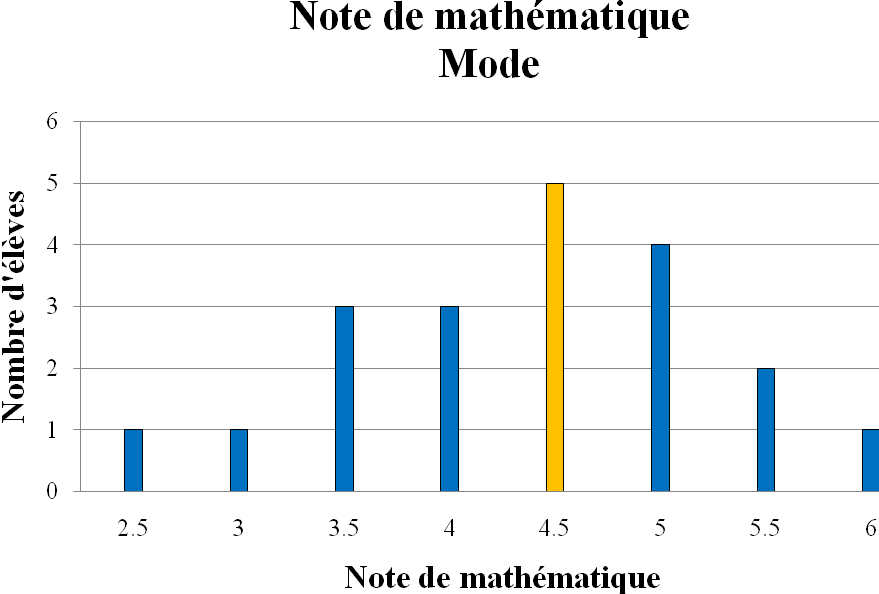
\includegraphics[width = 0.4 \textwidth]{statistiques/image/mode1.png} \hspace{5mm}
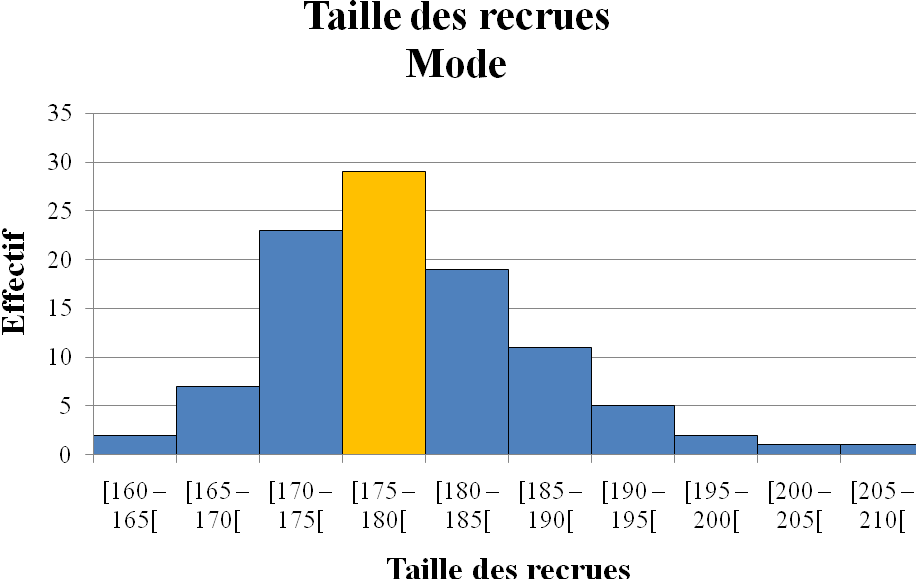
\includegraphics[width = 0.4 \textwidth]{statistiques/image/mode2.png} 
\end{center}

Et celle des fréquences cumulées met en évidence la médiane :
\begin{center}
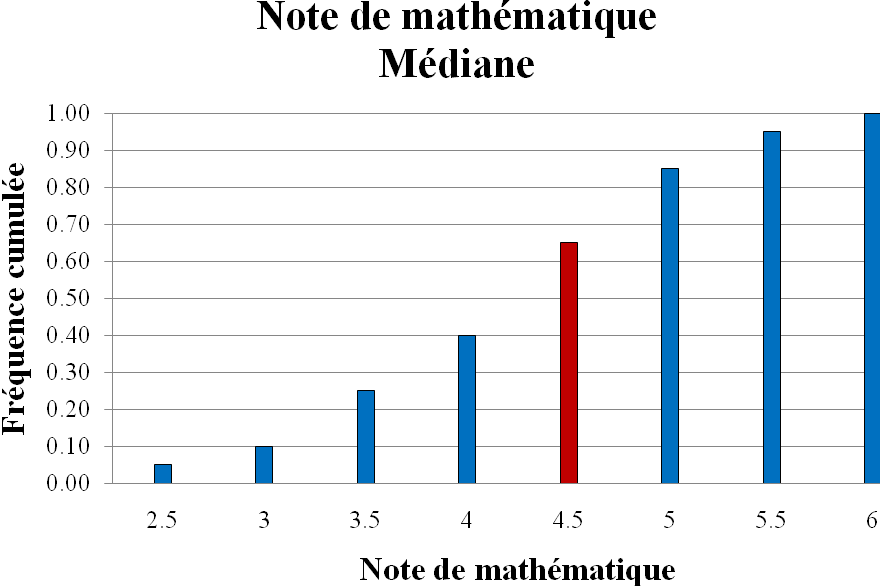
\includegraphics[width = 0.4 \textwidth]{statistiques/image/mediane1.png} \hspace{5mm}
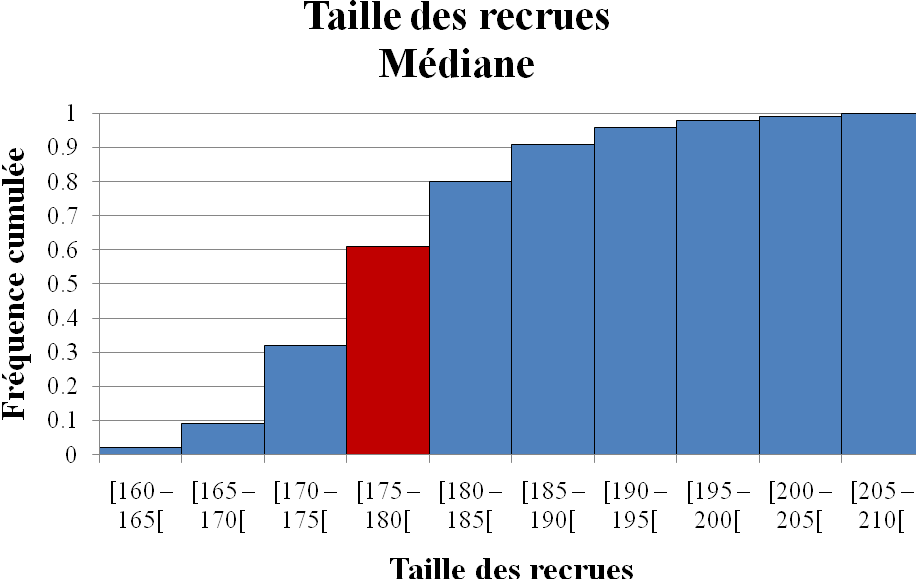
\includegraphics[width = 0.4 \textwidth]{statistiques/image/mediane2.png}
\end{center}

\section{Courbe de régression}

Pour l'instant, nous ne nous somme intéressés qu'à des distributions statistiques univariées, c'est-à-dire avec un seul caractère. Or souvent il est intéressant de savoir comment plusieurs caractères s'influencent. On parle alors de statistiques bivariées~\index{statistiques!bivariées}. 

Lors de notre distribution, chaque observation est représentée comme un point sur le plan, la coordonnée $x$ étant la valeur de la première variable et la coordonnée $y$ la valeur de la deuxième variable.

On obtient donc un nuage de points. S'il y a un lien entre les points, qu'on peut y faire passer une courbe, on va parler de \emph{régression}. 

\begin{center}
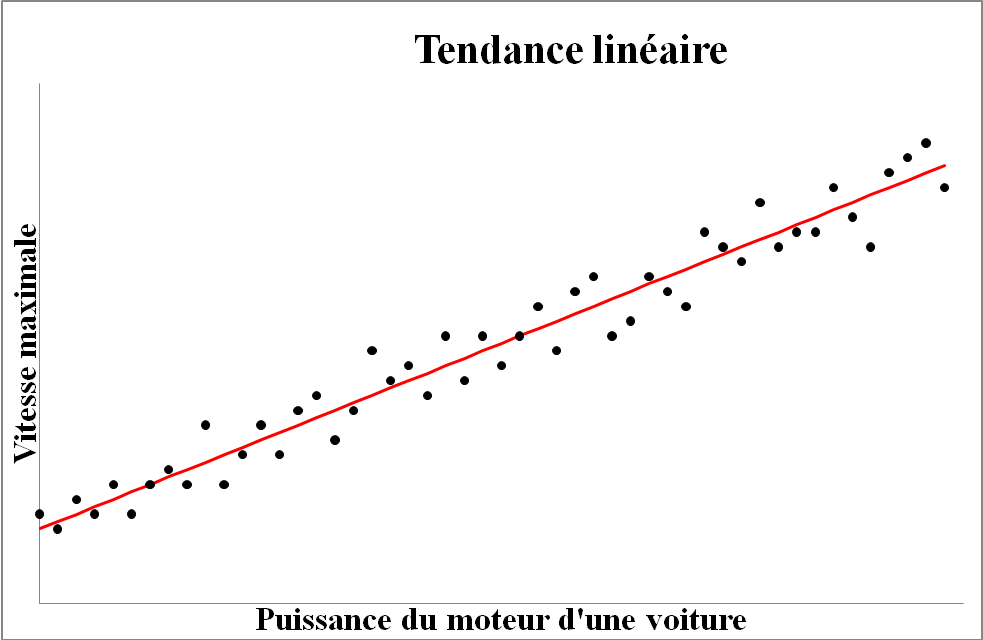
\includegraphics[width = 0.4 \textwidth]{statistiques/image/regression1.png} \hspace{5mm}
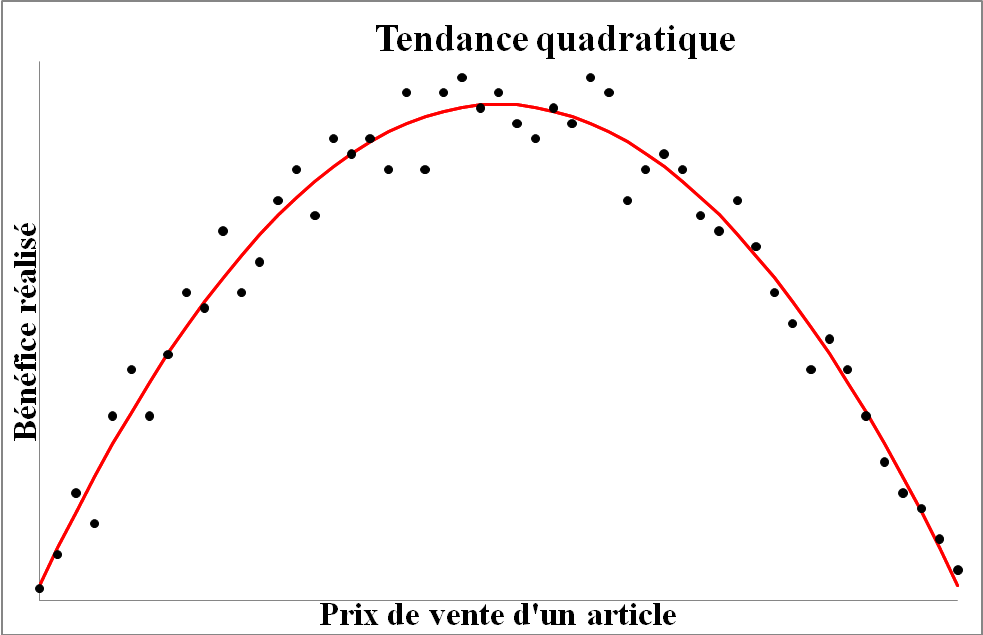
\includegraphics[width = 0.4 \textwidth]{statistiques/image/regression2.png}

\vspace{5mm}

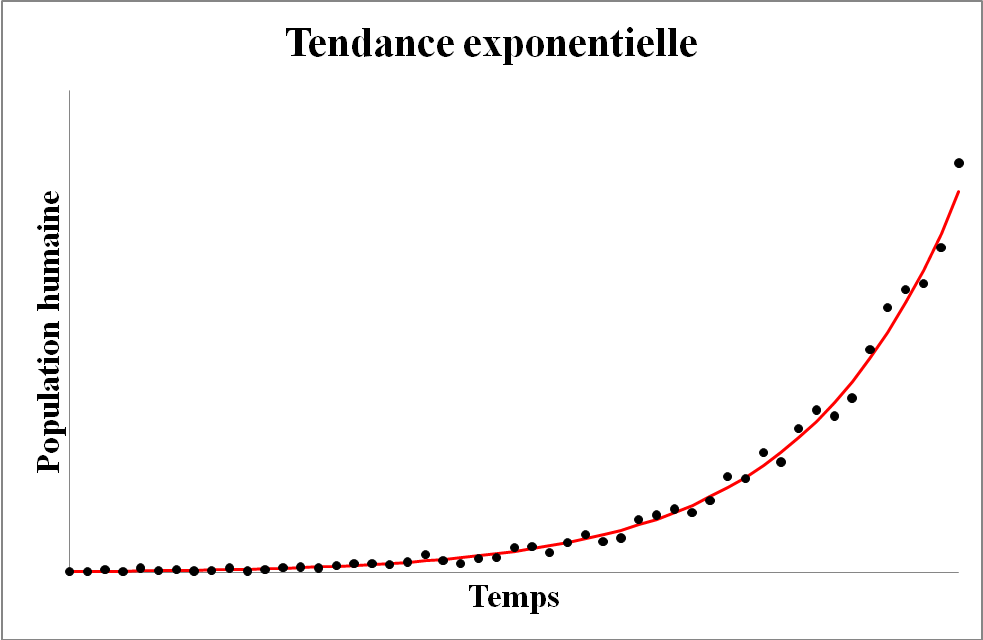
\includegraphics[width = 0.4 \textwidth]{statistiques/image/regression3.png} \hspace{5mm}
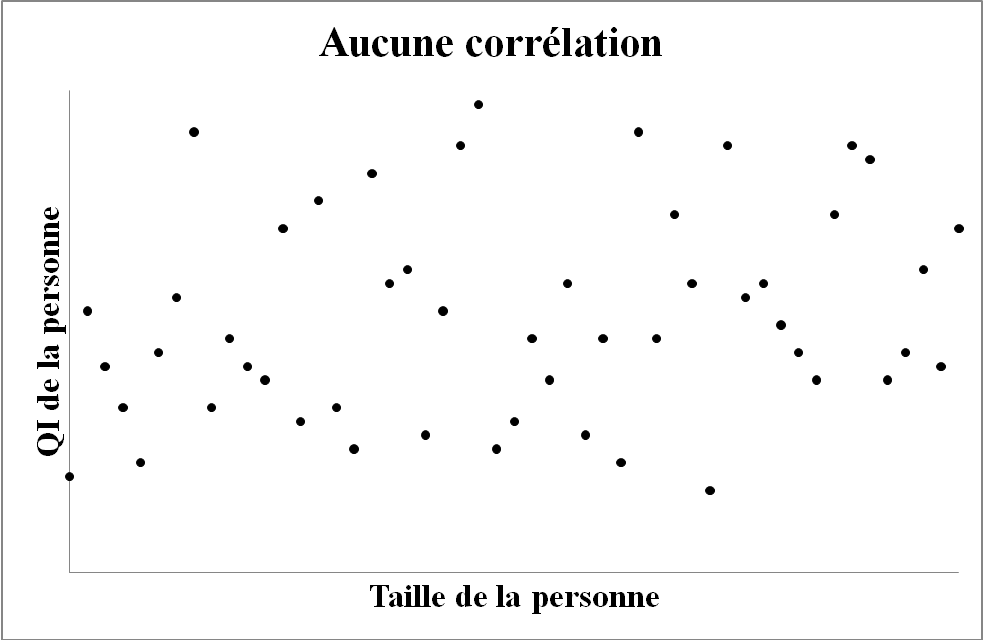
\includegraphics[width = 0.4 \textwidth]{statistiques/image/regression4.png}
\end{center}

\textcolor{red}{Attention : ce n'est pas parce qu'on peut faire passer une courbe par les points que forcément il y a un rapport de causalité entre les deux caractères !} Par exemple, le graphique suivant met en parallèle le nombre de Prix Nobel par million d'habitants et la consommation de chocolat en kg par habitant :
\begin{center}
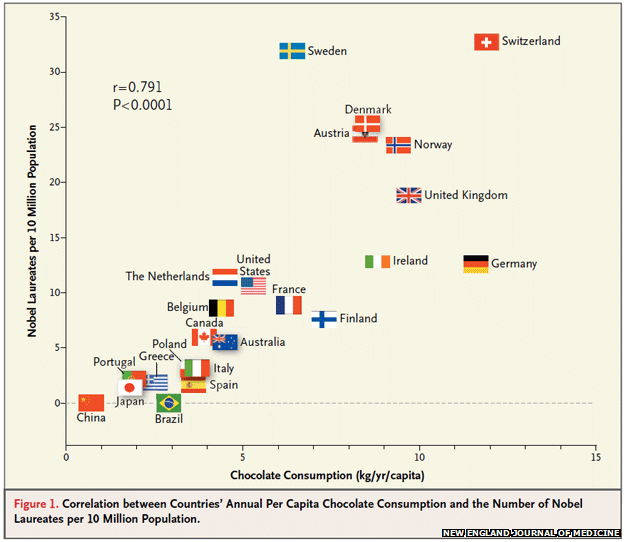
\includegraphics[width = 0.6\textwidth]{statistiques/image/chocolat.png}
\end{center}
Mais, par contre, il est évident qu'il n'y a pas de lien de causalité entre ces deux variables.

Dans les graphiques, il y a plusieurs manières de faire passer des courbes par le nuage de points. Cependant, nous ne nous intéresserons qu'au cas où l'on peut faire passer une droite de la forme
$$
y = ax+b
$$
où $a$ est la pente de la droite et $b$ l'intersection avec l'axe vertical.

Enfin, on note $r$ le coefficient de régression qui nous indique à quel point la droite passe près de chaque point. Si $r$ est supérieur à $0.5$ ou inférieur à $-0.5$, on dit que la corrélation est forte. Si $r$ est entre $-0.5$ et $0.5$, on parle de corrélation faible.

Pour calculer la valeur de $a$, de $b$ et de $r$, on doit également réaliser un tableau statistique contenant $5$ colonnes : 
\begin{enumerate}[colonne 1 :]
\item la valeur $x$ du point
\item la valeur $y$ correspondante
\item $x^2$
\item $y^2$
\item $xy$
\end{enumerate}

Pour chacune de ces colonnes, il faut calculer la moyenne, c'est-à-dire la somme des termes divisée par le nombre de mesures.

On a ainsi les formules suivantes, où par exemple $\overline{x}$ correspond à la moyenne de la colonne $x$ :
$$
a  = \frac{\overline{xy}-\overline{x}\cdot \overline{y}}{\overline{x^2}-\left(\overline{x}\right)^2}
$$

$$
b = \overline{y}-a\cdot \overline{x}
$$

$$
r = \frac{\overline{xy}- \overline{x}\cdot \overline{y}}{\sqrt{\overline{x^2}-\overline{x}^2} \cdot \sqrt{\overline{y^2}-\overline{y}^2}}
$$

\begin{exemple}

\begin{tabular}{|l|l|l|l|l|l|}
\hline
      & $x_i$ & $y_i$ & $(x_i)^2$ & $(y_i)^2$ & $x_i y_i$ \\
      \hline
      & 2  & 3  & 4     & 9     & 6    \\
      \hline
      & 2  & 5  & 4     & 25    & 10   \\
      \hline
      & 3  & 6  & 9     & 36    & 18   \\
      \hline
      & 4  & 5  & 16    & 25    & 20   \\
      \hline
      & 5  & 6  & 25    & 36    & 30   \\
      \hline
      & 5  & 7  & 25    & 49    & 35   \\
      \hline
      & 6  & 8  & 36    & 64    & 48   \\
      \hline
      & 7  & 9  & 49    & 81    & 63   \\
      \hline
      & 7  & 8  & 49    & 64    & 56   \\
      \hline
      & 8  & 9  & 64    & 81    & 72   \\
      \hline
      & 9  & 10 & 81    & 100   & 90   \\
      \hline
      & 10 & 12 & 100   & 144   & 120  \\
      \hline
Somme   & 68 & 88 & 462   & 714   & 568  \\
\hline
Moyenne &  5.66  &  7.33  &   38.5    &   59.5    &   47.33 \\ 
\hline
\end{tabular}

$$
a = \frac{47.33-5.66\cdot 7.33}{38.5 - 5.66^2} \simeq 0.904
$$

$$
b = 7.33 - 0.904 \cdot 5.6 \simeq 2.209
$$

$$
r = \frac{47.33-5.66\cdot 7.33}{\sqrt{38.5-5.66^2} \cdot \sqrt{59.5 - 7.33^2}}\simeq 0.956
$$

On a ainsi la courbe 
$$
y = 0.904 x + 2.209
$$
qui est bien corrélée ($0.956$) :

\begin{center}
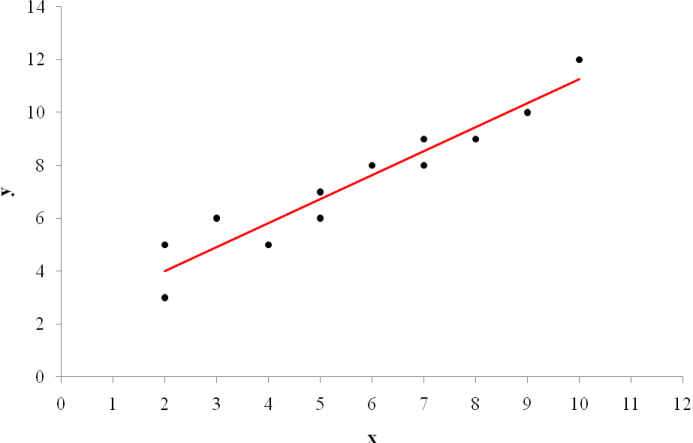
\includegraphics[width = 0.7\textwidth]{statistiques/image/regression10.png}
\end{center}

%calcul de a, b et r et droite de régression et schéma

\end{exemple}

\begin{remarque}[Le quartet d'Anscombe~\cite{wikianscombe}]
Il ne suffit pas toujours de simplement calculer les droites de régression pour bien visualiser une situation. L'exemple le plus connu est le quartet d'Anscombe~\index{Anscombe!quartet}. Il présente quatre ensembles de données qui paraissent similaires mais qui sont en réalité très différentes.

\begin{center}
\begin{tabular}{|ll|ll|ll|ll|}
\hline
I    &       & II   &      & III  &       & IV   &       \\
\hline
$x$    & $y$     & $x$    & $y$    & $x$    & $y$     & $x$    & $y$     \\
10,0 & 8,04  & 10,0 & 9,14 & 10,0 & 7,46  & 8,0  & 6,58  \\
8,0  & 6,95  & 8,0  & 8,14 & 8,0  & 6,77  & 8,0  & 5,76  \\
13,0 & 7,58  & 13,0 & 8,74 & 13,0 & 12,74 & 8,0  & 7,71  \\
9,0  & 8,81  & 9,0  & 8,77 & 9,0  & 7,11  & 8,0  & 8,84  \\
11,0 & 8,33  & 11,0 & 9,26 & 11,0 & 7,81  & 8,0  & 8,47  \\
14,0 & 9,96  & 14,0 & 8,10 & 14,0 & 8,84  & 8,0  & 7,04  \\
6,0  & 7,24  & 6,0  & 6,13 & 6,0  & 6,08  & 8,0  & 5,25  \\
4,0  & 4,26  & 4,0  & 3,10 & 4,0  & 5,39  & 19,0 & 12,50 \\
12,0 & 10,84 & 12,0 & 9,13 & 12,0 & 8,15  & 8,0  & 5,56  \\
7,0  & 4,82  & 7,0  & 7,26 & 7,0  & 6,42  & 8,0  & 7,91  \\
5,0  & 5,68  & 5,0  & 4,74 & 5,0  & 5,73  & 8,0  & 6,89 \\
\hline
\end{tabular}
\end{center}

Toutes ces distributions ont un coefficient de corrélation de $0.816$ et une droite de régression $y=3 + 0.5 x$, MAIS... lorsqu'on visualise les graphiques :

\begin{center}
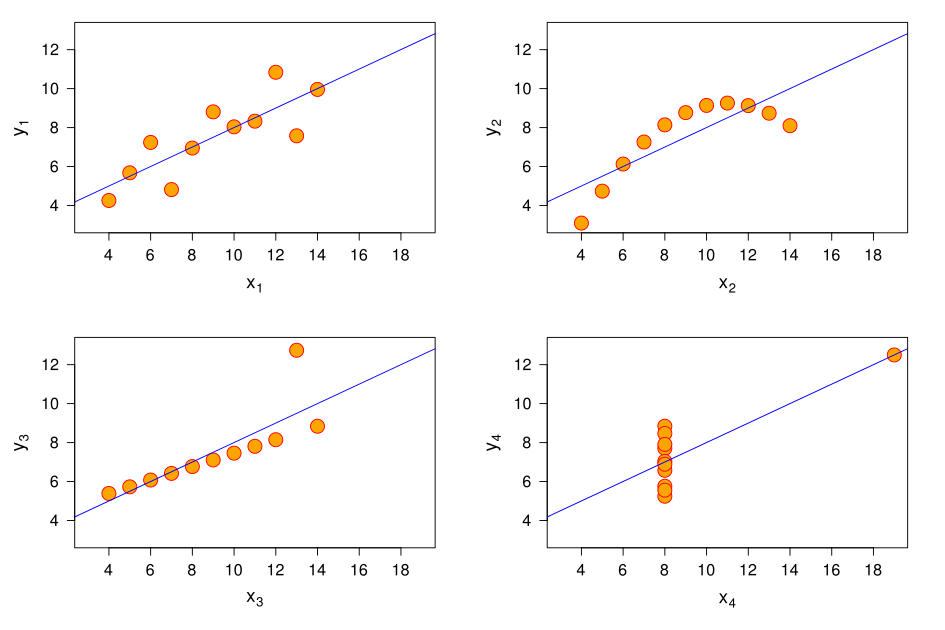
\includegraphics[width = 0.9\textwidth]{statistiques/image/anscombe.png}
\end{center}

La première distribution est un cas typique de données corrélées. La deuxième distribution suit clairement une corrélation quadratique, mais suffisamment proche. La troisième est parfaitement corrélée, mais une donnée aberrante fausse les calculs. Enfin la dernière montre qu'une erreur de mesure fait apparaître un coefficient de corrélation élevé alors que la variable $x$ est constante.

\end{remarque}


\section{Exercices}

\begin{exercice}
Voici le nombre de points obtenus dans une épreuve commune de mathématiques.

\begin{tabular}{|l|l|}
\hline
Nombre de points & Nombres d'élèves \\ \hline
10               & 2                \\ \hline
9                & 7                \\ \hline
8                & 11               \\ \hline
7                & 17               \\ \hline
6                & 14               \\ \hline
5                & 12               \\ \hline
4                & 8                \\ \hline
3                & 5                \\ \hline
2                & 3                \\ \hline
1                & 1                \\ \hline
\end{tabular}

Établir le tableau statistique complet. Précision des calculs dans le tableau : 4 chiffres après la virgule.
Établir l'histogramme des effectifs et des fréquences cumulées.
Indiquer le mode et la médiane de cette distribution statistique.
Calculer la moyenne et l'écart-type.
S'il faut avoir 6 points pour avoir la moyenne à cet examen, calculer le pourcentage d'élèves qui ont alors obtenu au minimum la note 4.
\end{exercice}

\begin{exercice}
On a relevé dans ce tableau la vitesse de 125 voitures sur l'autoroute.

\begin{tabular}{|l|l|l|l|l|l|l|l}
\hline
136 & 132 & 137 & 120 & 130 & 108 & 147 & \multicolumn{1}{l|}{136} \\ \hline
142 & 134 & 109 & 120 & 130 & 128 & 142 & \multicolumn{1}{l|}{131} \\ \hline
142 & 135 & 105 & 95  & 131 & 98  & 127 & \multicolumn{1}{l|}{116} \\ \hline
156 & 111 & 114 & 108 & 133 & 118 & 108 & \multicolumn{1}{l|}{146} \\ \hline
120 & 127 & 106 & 132 & 98  & 163 & 115 & \multicolumn{1}{l|}{117} \\ \hline
117 & 167 & 127 & 135 & 113 & 115 & 124 & \multicolumn{1}{l|}{118} \\ \hline
132 & 110 & 114 & 134 & 115 & 134 & 112 & \multicolumn{1}{l|}{141} \\ \hline
135 & 124 & 119 & 175 & 119 & 102 & 151 & \multicolumn{1}{l|}{128} \\ \hline
116 & 114 & 118 & 111 & 129 & 133 & 130 & \multicolumn{1}{l|}{125} \\ \hline
124 & 124 & 123 & 118 & 105 & 120 & 123 & \multicolumn{1}{l|}{118} \\ \hline
148 & 126 & 116 & 113 & 112 & 117 & 134 & \multicolumn{1}{l|}{106} \\ \hline
119 & 107 & 143 & 140 & 128 & 131 & 137 & \multicolumn{1}{l|}{122} \\ \hline
123 & 125 & 160 & 157 & 99  & 116 & 120 & \multicolumn{1}{l|}{117} \\ \hline
125 & 152 & 108 & 121 & 115 & 125 & 145 &                          \\ \cline{1-7}
110 & 153 & 107 & 132 & 128 & 98  & 116 &                          \\ \cline{1-7}
122 & 121 & 145 & 116 & 102 & 125 & 125 &                          \\ \cline{1-7}
\end{tabular}

On demande de trier les résultats en classe de 10 km/h, puis de recopier et de compléter le tableau ci-dessous.

\begin{landscape}

\begin{tabular}{llllllll}
\cline{1-1}
\multicolumn{1}{|l|}{\begin{tabular}{l}Vitesse mesurée (en km/h)\\ de 125 véhicules \\ sur l'autoroute\end{tabular}} &                                &                                &                                &                                &                                  &                                &                                   \\ \hline
\multicolumn{1}{|l|}{Classes}                                                    & \multicolumn{1}{l|}{Centre}    & \multicolumn{1}{l|}{Effectifs} & \multicolumn{1}{l|}{Fréquence} & \multicolumn{1}{l|}{Fréquence} & \multicolumn{1}{l|}{Fréquence}   & \multicolumn{1}{l|}{Fréquence} & \multicolumn{1}{l|}{Fréquence}    \\ \hline
\multicolumn{1}{|l|}{(en km/h)}                                                  & \multicolumn{1}{l|}{de classe} & \multicolumn{1}{l|}{}          & \multicolumn{1}{l|}{}          & \multicolumn{1}{l|}{cumulée}   & \multicolumn{1}{l|}{cumulée inv} & \multicolumn{1}{l|}{pondérée}  & \multicolumn{1}{l|}{pond. carrée} \\ \hline
\multicolumn{1}{|l|}{{]}90 - 100{]}}                                             & \multicolumn{1}{l|}{}          & \multicolumn{1}{l|}{}          & \multicolumn{1}{l|}{}          & \multicolumn{1}{l|}{}          & \multicolumn{1}{l|}{}            & \multicolumn{1}{l|}{}          & \multicolumn{1}{l|}{}             \\ \hline
\multicolumn{1}{|l|}{{]}100 - 110{]}}                                            & \multicolumn{1}{l|}{}          & \multicolumn{1}{l|}{}          & \multicolumn{1}{l|}{}          & \multicolumn{1}{l|}{}          & \multicolumn{1}{l|}{}            & \multicolumn{1}{l|}{}          & \multicolumn{1}{l|}{}             \\ \hline
\multicolumn{1}{|l|}{{]}110 - 120{]}}                                            & \multicolumn{1}{l|}{}          & \multicolumn{1}{l|}{}          & \multicolumn{1}{l|}{}          & \multicolumn{1}{l|}{}          & \multicolumn{1}{l|}{}            & \multicolumn{1}{l|}{}          & \multicolumn{1}{l|}{}             \\ \hline
\multicolumn{1}{|l|}{{]}120 - 130{]}}                                            & \multicolumn{1}{l|}{}          & \multicolumn{1}{l|}{}          & \multicolumn{1}{l|}{}          & \multicolumn{1}{l|}{}          & \multicolumn{1}{l|}{}            & \multicolumn{1}{l|}{}          & \multicolumn{1}{l|}{}             \\ \hline
\multicolumn{1}{|l|}{{]}130 - 140{]}}                                            & \multicolumn{1}{l|}{}          & \multicolumn{1}{l|}{}          & \multicolumn{1}{l|}{}          & \multicolumn{1}{l|}{}          & \multicolumn{1}{l|}{}            & \multicolumn{1}{l|}{}          & \multicolumn{1}{l|}{}             \\ \hline
\multicolumn{1}{|l|}{{]}140 - 150{]}}                                            & \multicolumn{1}{l|}{}          & \multicolumn{1}{l|}{}          & \multicolumn{1}{l|}{}          & \multicolumn{1}{l|}{}          & \multicolumn{1}{l|}{}            & \multicolumn{1}{l|}{}          & \multicolumn{1}{l|}{}             \\ \hline
\multicolumn{1}{|l|}{{]}150 - 160{]}}                                            & \multicolumn{1}{l|}{}          & \multicolumn{1}{l|}{}          & \multicolumn{1}{l|}{}          & \multicolumn{1}{l|}{}          & \multicolumn{1}{l|}{}            & \multicolumn{1}{l|}{}          & \multicolumn{1}{l|}{}             \\ \hline
\multicolumn{1}{|l|}{{]}160 - 170{]}}                                            & \multicolumn{1}{l|}{}          & \multicolumn{1}{l|}{}          & \multicolumn{1}{l|}{}          & \multicolumn{1}{l|}{}          & \multicolumn{1}{l|}{}            & \multicolumn{1}{l|}{}          & \multicolumn{1}{l|}{}             \\ \hline
\multicolumn{1}{|l|}{{]}170 - 180{]}}                                            & \multicolumn{1}{l|}{}          & \multicolumn{1}{l|}{}          & \multicolumn{1}{l|}{}          & \multicolumn{1}{l|}{}          & \multicolumn{1}{l|}{}            & \multicolumn{1}{l|}{}          & \multicolumn{1}{l|}{}             \\ \hline
                                                                                 & \multicolumn{1}{l|}{}          & \multicolumn{1}{l|}{}          & \multicolumn{1}{l|}{}          &                                & \multicolumn{1}{l|}{}            & \multicolumn{1}{l|}{}          & \multicolumn{1}{l|}{}             \\ \cline{3-4} \cline{7-8} 
\end{tabular}

\end{landscape}

Établir l'histogramme des fréquences et des fréquences cumulées.
Indiquer la valeur de la classe modale et de la classe médiane.
Calculer la vitesse moyenne et l'écart-type.
Calculer le pourcentage de véhicules qui roulent à une vitesse supérieure à la vitesse autorisée en Suisse.
\end{exercice}

\begin{exercice}
Afin d'analyser les habitudes de la clientèle d’un supermarché, le gérant a relevé les montants des achats faits par les clients un lundi après-midi et un samedi après-midi.

\begin{tabular}{lll|l|l|}
\cline{1-2} \cline{4-5}
\multicolumn{1}{|l|}{Lundi aprčs-midi} & \multicolumn{1}{l|}{}         &  & Samedi aprčs-midi &          \\ \cline{1-2} \cline{4-5} 
\multicolumn{1}{|l|}{Classe}           & \multicolumn{1}{l|}{Effectif} &  & Classe            & Effectif \\ \cline{1-2} \cline{4-5} 
\multicolumn{1}{|l|}{{]}0 - 20{]}}     & \multicolumn{1}{l|}{7}        &  & {]}0 - 20{]}      & 5        \\ \cline{1-2} \cline{4-5} 
\multicolumn{1}{|l|}{{]}20 - 40{]}}    & \multicolumn{1}{l|}{16}       &  & {]}20 - 40{]}     & 12       \\ \cline{1-2} \cline{4-5} 
\multicolumn{1}{|l|}{{]}40 - 60{]}}    & \multicolumn{1}{l|}{32}       &  & {]}40 - 60{]}     & 23       \\ \cline{1-2} \cline{4-5} 
\multicolumn{1}{|l|}{{]}60 - 80{]}}    & \multicolumn{1}{l|}{24}       &  & {]}60 - 80{]}     & 48       \\ \cline{1-2} \cline{4-5} 
\multicolumn{1}{|l|}{{]}80 - 100{]}}   & \multicolumn{1}{l|}{10}       &  & {]}80 - 100{]}    & 61       \\ \cline{1-2} \cline{4-5} 
\multicolumn{1}{|l|}{{]}100 - 120{]}}  & \multicolumn{1}{l|}{7}        &  & {]}100 - 120{]}   & 34       \\ \cline{1-2} \cline{4-5} 
\multicolumn{1}{|l|}{{]}120 - 140{]}}  & \multicolumn{1}{l|}{3}        &  & {]}120 - 140{]}   & 29       \\ \cline{1-2} \cline{4-5} 
\multicolumn{1}{|l|}{{]}140 - 160{]}}  & \multicolumn{1}{l|}{1}        &  & {]}140 - 160{]}   & 14       \\ \cline{1-2} \cline{4-5} 
                                       &                               &  & {]}160 - 180{]}   & 12       \\ \cline{4-5} 
                                       &                               &  & {]}180 - 200{]}   & 6        \\ \cline{4-5} 
                                       &                               &  & {]}200 - 220{]}   & 4        \\ \cline{4-5} 
                                       &                               &  & {]}220 - 240{]}   & 2        \\ \cline{4-5} 
\end{tabular}

Il te demande d'établir, pour chaque après-midi étudiée, un tableau statistique (montants des achats groupés en classes de vingt francs), de calculer le mode, la médiane, la moyenne des dépenses et l'écart-type. Il souhaite aussi connaître le pourcentage des clients dont le montant des achats est égal ou inférieur à Fr. 60.–– et le pourcentage de ceux dont le montant est strictement supérieur à Fr. 100.—. Précision des calculs : trois chiffres après la virgule.
Avec les résultats obtenus, le gérant du supermarché te demande encore de faire, pour chaque après-midi, un commentaire sur les habitudes d'achat de la clientèle (justifier les commentaires en utilisant les divers paramètres statistiques calculés !). Il souhaite aussi que tu trouves quelques raisons sociologiques aux différences observées.
\end{exercice}

\begin{exercice}
On a mesuré la longueur en millimètres des grains de deux variétés de riz. Les résultats des mesures ont été répertoriés dans le tableau annexé.

\begin{tabular}{|l|l|l|}
\hline
                         & Variété A & Variété B \\ \hline
Taille des grains de riz & Effectif  & Effectif  \\ \hline
{]}0  2{]}               & 7         & 2         \\ \hline
{]}2 - 4{]}              & 37        & 5         \\ \hline
{]}4 - 6{]}              & 72        & 28        \\ \hline
{]}6 - 8{]}              & 89        & 98        \\ \hline
{]}8 - 10{]}             & 97        & 230       \\ \hline
{]}10 - 12{]}            & 91        & 107       \\ \hline
{]}12 - 14{]}            & 69        & 25        \\ \hline
{]}14 - 16{]}            & 34        & 4         \\ \hline
{]}16 - 18{]}            & 4         & 1         \\ \hline
\end{tabular}

\begin{enumerate}
\item Pour chaque variété de riz, établir un tableau de statistiques complet. 
	Précision des calculs : trois chiffres après la virgule.
\item Pour chacune des deux variétés de riz, on souhaite connaître :
	\begin{itemize}
	\item La classe modale,
	\item Le pourcentage des effectifs que représente la classe modale à elle seule,
	\item Le pourcentage des grains ayant une mesure inférieure ou égale à 8 mm,
	\item Le pourcentage des grains ayant une mesure strictement supérieure à 10 mm,
	\item La classe médiane,
	\item La moyenne,
	\item L’écart-type.
	\end{itemize}
\item Procéder à une analyse des résultats statistiques obtenus puis comparer les deux variétés de riz.
\item Pour commercialiser le riz, on procède à un tri mécanique qui élimine à la fois les grains dont la taille est inférieure ou égale à 6 millimètres et les grains dont la taille est strictement supérieure à 14 millimètres. Quelle variété de riz se prêtera le mieux à la commercialisation, justifier votre réponse ? 
\end{enumerate}
\end{exercice}


\begin{exercice}
Voici trois exemples de distribution statistique. Commenter chacune de ces distributions avec les renseignements fournis par les histogrammes, les modes, les médianes, les moyennes et les écarts-types. Donner un exemple d''étude d'un caractère d'une population qui aurait le même genre de distribution.
\begin{center}
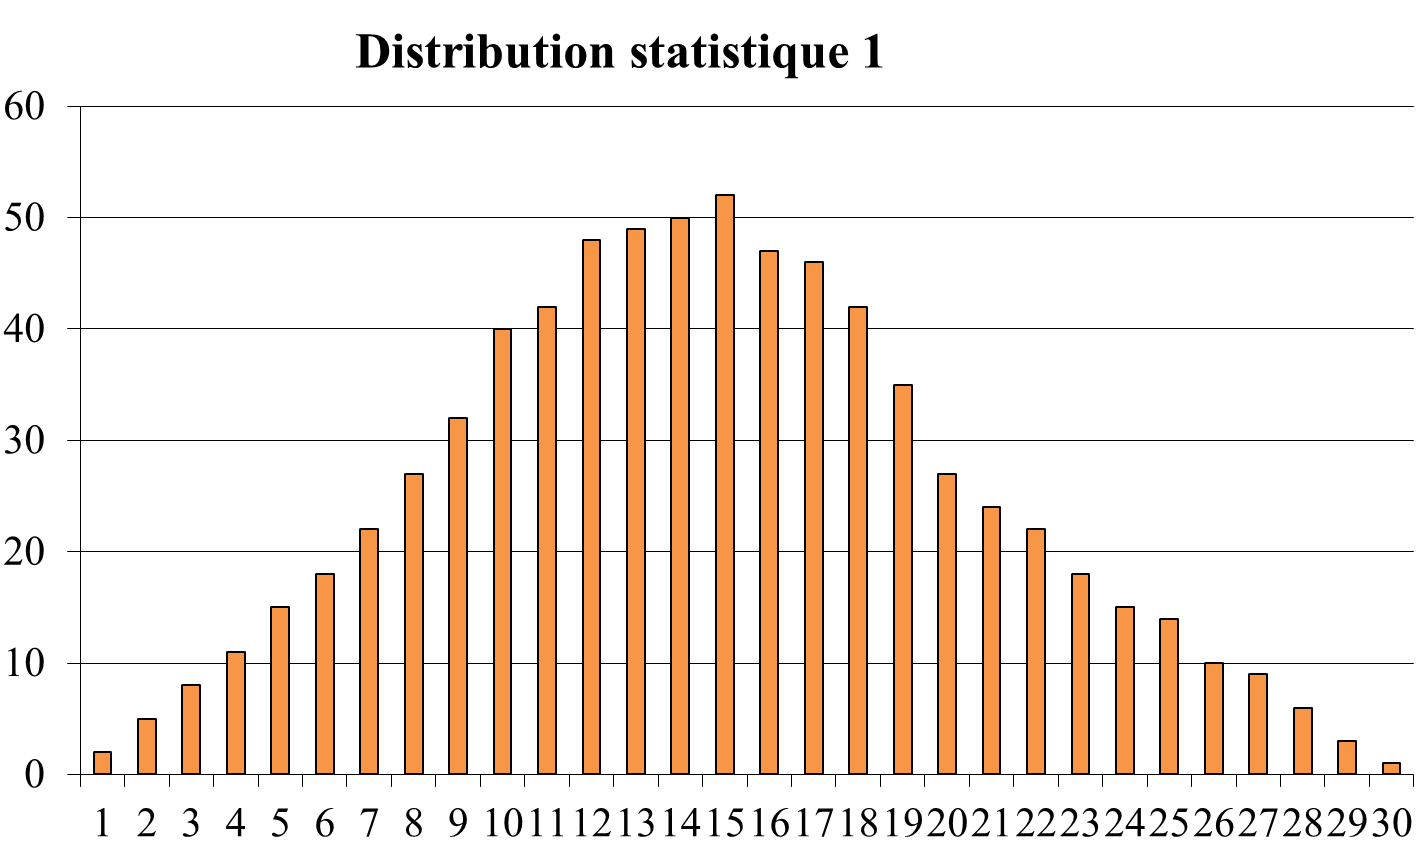
\includegraphics[width = 0.5\textwidth]{statistiques/image/graphique1.png}
\end{center}
Mode : 15
Médiane : 15
Moyenne : 14.69
Écart-type : 5.78
\begin{center}
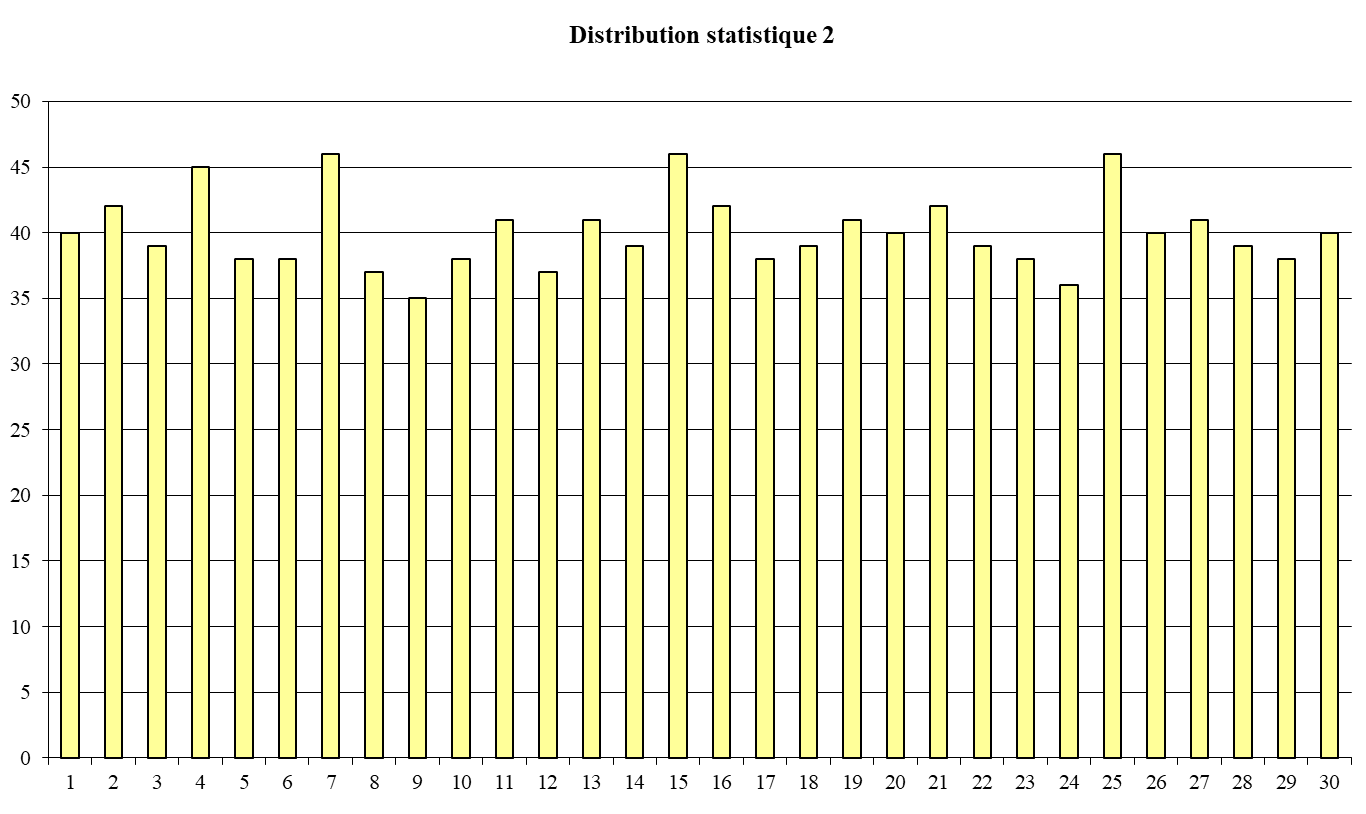
\includegraphics[width = 0.5\textwidth]{statistiques/image/graphique2.png}
\end{center}
Mode : 5
Médiane : 13
Moyenne : 14.77
Écart-type : 9.44
\begin{center}
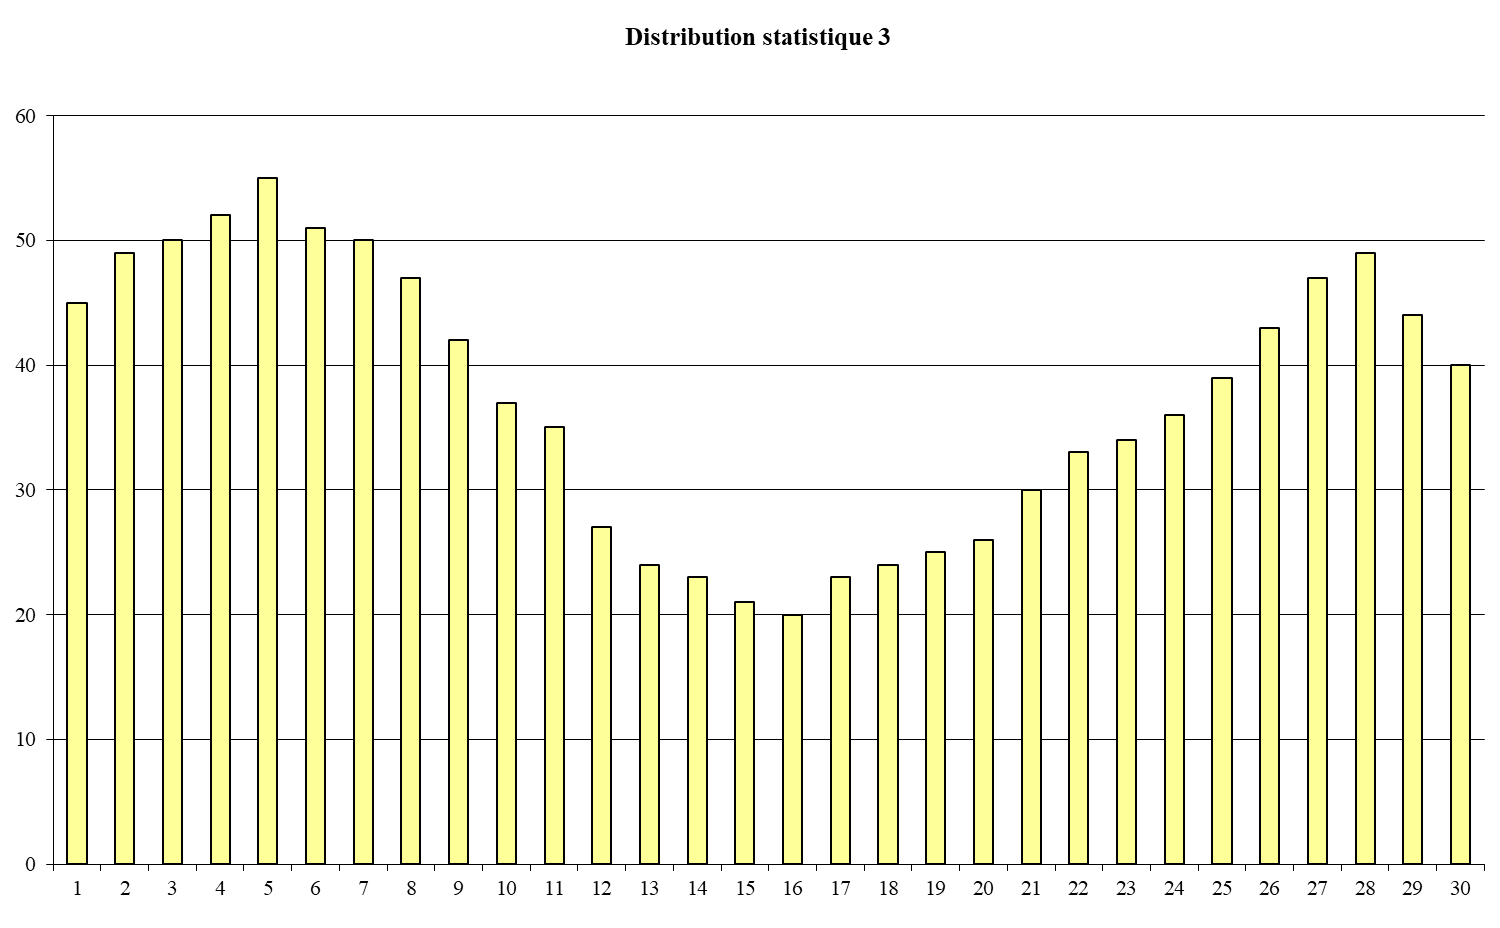
\includegraphics[width = 0.5\textwidth]{statistiques/image/graphique3.png}
\end{center}
Mode : 7 – 15 - 25
Médiane : 15
Moyenne : 15.47
Écart-type : 8.66
\end{exercice}

\begin{exercice}
Dans le tableau suivant, on a répertorié le nombre de repas servis à midi dans un restaurant. Calculer l'équation de la droite de régression linéaire et le coefficient de corrélation. Commenter les résultats obtenus.

\begin{tabular}{|l|l|l|l|l|l|l|l|}
\cline{1-2} \cline{4-5} \cline{7-8}
Jour (x) & Repas (y) &  & Jour (x) & Repas (y) &  & Jour (x) & Repas(y) \\ \cline{1-2} \cline{4-5} \cline{7-8} 
1        & 12        &  & 11       & 16        &  & 21       & 31       \\ \cline{1-2} \cline{4-5} \cline{7-8} 
2        & 10        &  & 12       & 15        &  & 22       & 22       \\ \cline{1-2} \cline{4-5} \cline{7-8} 
3        & 13        &  & 13       & 17        &  & 23       & 24       \\ \cline{1-2} \cline{4-5} \cline{7-8} 
4        & 12        &  & 14       & 25        &  & 24       & 15       \\ \cline{1-2} \cline{4-5} \cline{7-8} 
5        & 11        &  & 15       & 15        &  & 25       & 23       \\ \cline{1-2} \cline{4-5} \cline{7-8} 
6        & 14        &  & 16       & 18        &  & 26       & 24       \\ \cline{1-2} \cline{4-5} \cline{7-8} 
7        & 20        &  & 17       & 20        &  & 27       & 21       \\ \cline{1-2} \cline{4-5} \cline{7-8} 
8        & 13        &  & 18       & 16        &  & 28       & 33       \\ \cline{1-2} \cline{4-5} \cline{7-8} 
9        & 8         &  & 19       & 22        &  & 29       & 19       \\ \cline{1-2} \cline{4-5} \cline{7-8} 
10       & 15        &  & 20       & 20        &  & 30       & 24       \\ \cline{1-2} \cline{4-5} \cline{7-8} 
\end{tabular}
\end{exercice}

\begin{exercice}
Un exploitant d'une épicerie pense qu'il existe une relation linéaire entre le nombre de clients et le jour de la semaine. Calculer l'équation de la droite de régression linéaire, le coefficient de corrélation, puis confirmer ou infirmer l'impression de l'exploitant.

\begin{tabular}{|l|l|l|l|l|l|l|l|}
\hline
Jour (x)              & Lundi & Mardi & Mercredi & Jeudi & Vendredi & Samedi & Dimanche \\ \hline
Nombre de clients (y) & 146   & 206   & 146      & 133   & 156      & 202    & 124      \\ \hline
\end{tabular}
\end{exercice}

\begin{exercice}
Le tableau suivant donne le prix de vente x (en francs) et la quantité y vendue d'un objet au cours des douze derniers mois.

\begin{tabular}{|l|l|l|l|l|l|l|l|l|l|l|l|l|}
\hline
Prix (x)     & 6  & 5  & 4   & 6  & 8  & 4   & 7  & 5   & 6  & 9  & 3   & 3   \\ \hline
Quantité (y) & 75 & 92 & 102 & 85 & 60 & 115 & 70 & 105 & 88 & 30 & 141 & 127 \\ \hline
\end{tabular}


Calculer l'équation de la droite de régression linéaire et le coefficient de corrélation linéaire.
Représenter le nuage de points et la droite de régression sur un même graphique. 
Unité des axes : abscisse 1 cm pour un franc, ordonnée 1 cm pour 10 objets
Selon ce modèle de régression, quel serait la quantité d'objets vendus pour un prix de vente de Fr. 10.— ?
Selon ce modèle de régression, à quel prix correspondrait une vente de 100 objets ?
\end{exercice}
